\documentclass{beamer}
\usetheme{Madrid}
\usepackage[utf8]{inputenc}
\usepackage[T1]{fontenc}
\usepackage{graphicx}
\usepackage{lmodern}
\usepackage{tikz}

% Pour enlever le \institute du bas de page
% Rapetisser les noms et date etc dans le footer
\setbeamertemplate{footline}
{
	\leavevmode%
	\hbox{%
	\begin{beamercolorbox}[wd=.333333\paperwidth,ht=2.25ex,dp=1ex,center]{author in head/foot}%
	\
	\end{beamercolorbox}%
	\begin{beamercolorbox}[wd=.333333\paperwidth,ht=2.25ex,dp=1ex,center]{title in head/foot}%
	\usebeamerfont{title in head/foot}\insertshorttitle
	\end{beamercolorbox}%
	\begin{beamercolorbox}[wd=.333333\paperwidth,ht=2.25ex,dp=1ex,right]{date in head/foot}%
	\usebeamerfont{date in head/foot}\insertshortdate{}\hspace*{2em}
	\insertframenumber{} / \inserttotalframenumber\hspace*{2ex} 
	\end{beamercolorbox}}%
	\vskip0pt%
}

\AtBeginSection[]
{
	\begin{frame}
		\tableofcontents[currentsection,hideallsubsections]
	\end{frame}
}

\title{Tableau virtuel interactif}
\author{Baptiste Saleil, Geoffrey Mélia, Julien Pagès, Kevin Bollini \\ \ \\Tuteur de projet: M. Puech}
\date{30 avril 2012}

\begin{document}
	\begin{frame}
		\titlepage
	\end{frame}

	\section{Introduction}
		\begin{frame}{Introduction}
		\begin{center}
		\LARGE{Ter de Master 1 : Tableau virtuel interactif} \\
		\large{Tuteur de projet: W. Puech}
		\end{center}
		
		But du projet :
		\begin{itemize}
      \item Proposer un sujet en lien avec nos deux formations
		\item Concevoir une application utilisant les mouvements de l'utilisateur (sans souris)
		\item Développer une bibliothèque de détection d'objet dans une image
		\item Exploiter cette bibliothèque pour reconnaitre les mouvements de l'utilisateur
		\item Pouvoir écrire ou dessiner à plusieurs sur un tableau virtuel
		\end{itemize}
		
		\end{frame}

	\begin{frame}{Vidéo de présentation}
		inclure la vidéo?
	\end{frame}

%Plan
	\begin{frame}{Plan}
		\tableofcontents
	\end{frame}
		
	\section{Analyse et Conception}
	\subsection{Choix de conceptions}
		\begin{frame}{Choix de conceptions}
			\begin{block}{Choix principaux}
				Découper le projet en deux parties distinctes : \\
				- une bibliothèque de suivi d'objets réutilisable \\
				- une application avec une interface naturelle exploitant cette bibliothèque \\
			\end{block}
		\end{frame}
		
	% Julien
	\subsection{Gestion de projet}
		\begin{frame}{Gestion de projet}
			\begin{block}{Méthodologie :}
			\begin{itemize}
			\item Se renseigner, réaliser une architecture de qualité
			\item Répartir le travail en fonction des compétences et formations de chacun
			\item Développer rapidement un prototype
			\item Développement incrémental en ajoutant des fonctionnalités
			\end{itemize}
			\end{block}
		\end{frame}
		
		\begin{frame}{Gestion de projet}
			\begin{block}{Organisation :}
			\begin{itemize}
				\item{Réunions}
				\item{Deux sous-groupes}
				\item{Partage des tâches au sein des groupes}
				\item{Décisions communes (à quatre)}
			\end{itemize}
			\end{block}
		
		\begin{block}{Collaboration :}
			\begin{itemize}
				\item{Gestionnaire de version (Subversion)}
				\item{Partage de documents (Mail et Subversion)}
				\item{Discussions (Mails / Instantanée)}
				\item{Édition collaborative pour le travail à distance (Gobby)}
			\end{itemize}
         \end{block}
		\end{frame}
		
	% Partie de Kevin
	\subsection{Analyse}
		\begin{frame}{Analyse}
			\begin{exampleblock}{Objectifs}
				\begin{itemize}
					\item{Identifier les besoins et envies des utilisateurs}
					\item{Distinguer et classer les fonctionnalités de l'application}
					\item{Établir un schéma de conception dans le temps}
					\item{Faciliter le développement, avoir des buts concrets}
					\item{Produire une application réellement aboutie}
				\end{itemize}
			\end{exampleblock}
		\end{frame}
	
	\subsection{Planning}
		\begin{frame}{Rétroplanning}	
			Rétroplanning (Diagramme de gantt) :
			\begin{center}
			% TODO : mettre à jour le rétroplanning
			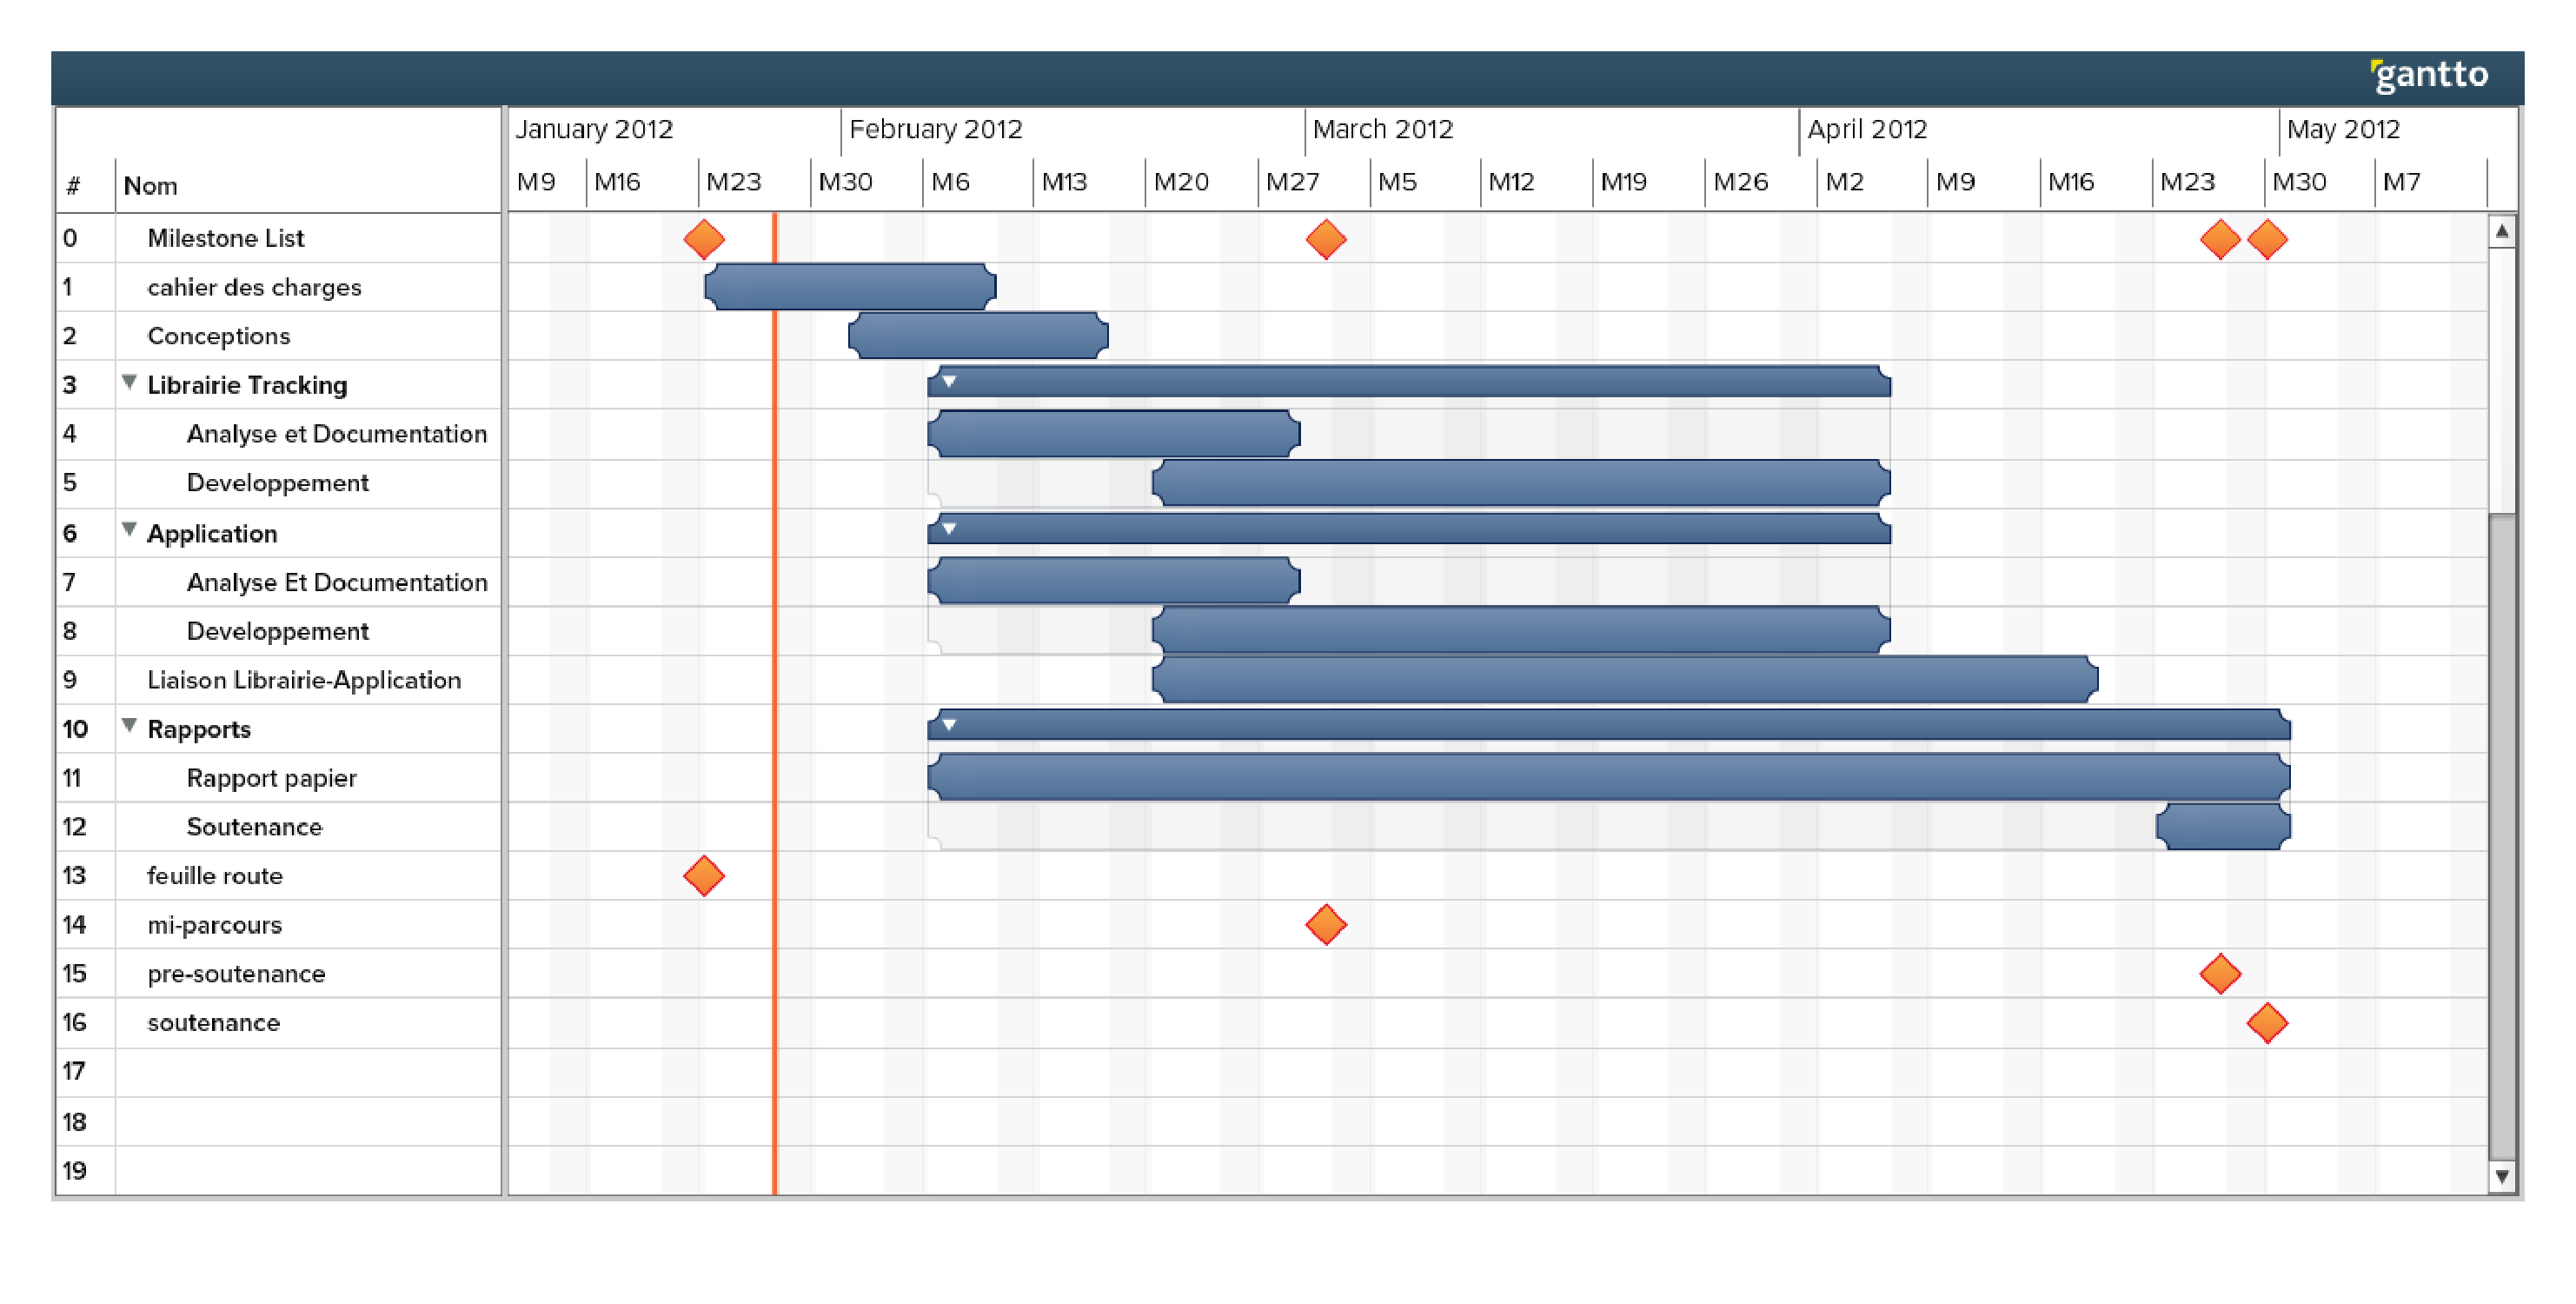
\includegraphics[scale=0.25]{../feuille-route/retroplanning.pdf}
			\end{center}
		\end{frame}
	
	% Geoffrey
	\section{Bibliothèque}
		\begin{frame}{Bibliothèque de suivi d'objets}
			\begin{block}{Objectifs de la bibliothèque conçue}
				\begin{itemize}
				\item{Distinguer complètement le suivi d'objet de l'application}
				\item{Avoir une utilisation simple sans connaissance en traitement d'image}
				\item{Permettre une détection d'action}
				\item{Proposer un maximum de solutions de suivi}
				\item{Évaluer et comparer ces solutions}
				\end{itemize}
			\end{block}
		\end{frame}

		\begin{frame}{Bibliothèque}
			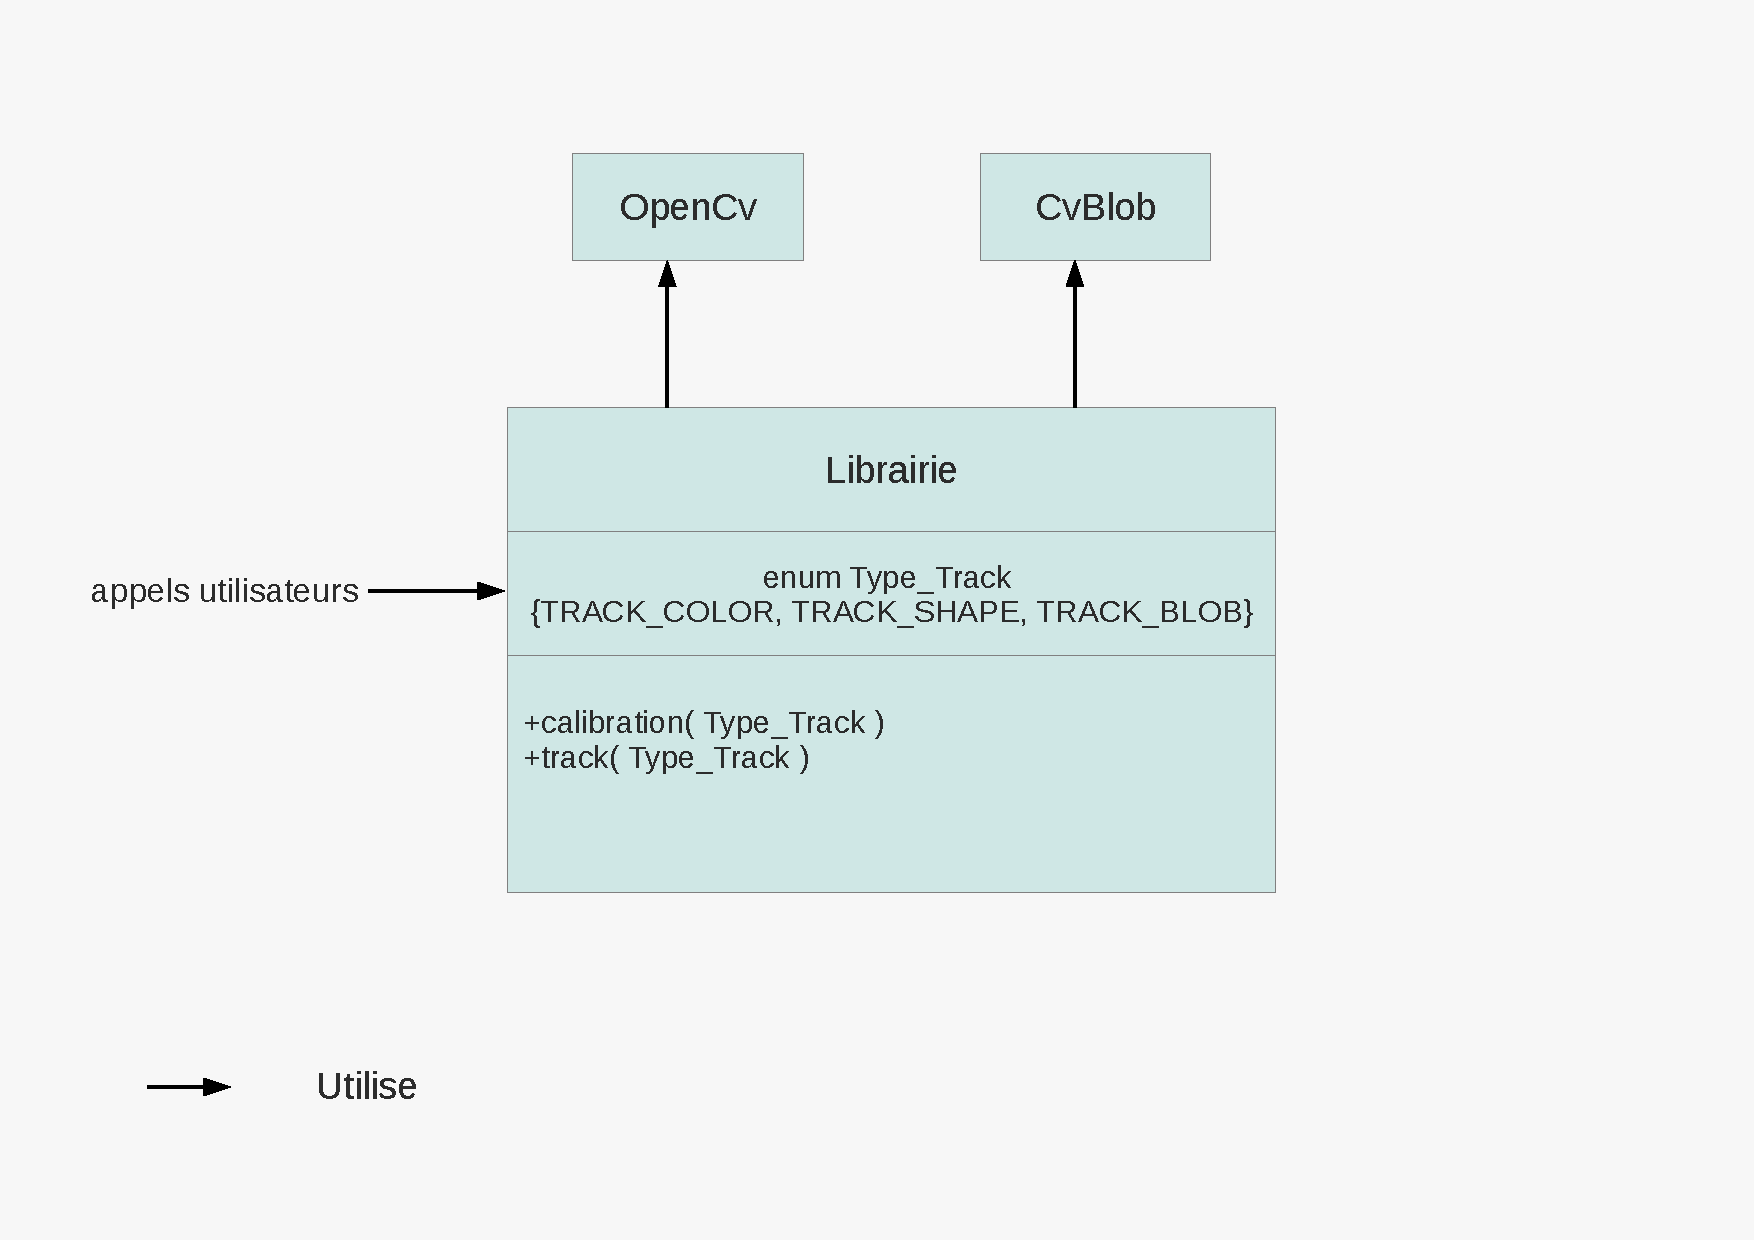
\includegraphics[scale=0.40]{schema-librairie.pdf}
		\end{frame}

		\begin{frame}{Bibliothèque}

		Création d'une structure de données : Cursor\\
		struct Cursor \{
		\begin{itemize}
			\item{CvPoint center}
			\item{CvPoint cornerA}
			\item{CvPoint cornerB}
			\item{...}
			\item{IplImage *mask}
			\item{Bool active}
		\end{itemize}
		\} \\
		\end{frame}
		
		\begin{frame}{Bibliothèque}
		Deux fonctions enveloppes : \\
			\begin{itemize}
				\item{Cursor * calibration(IplImage * source, CvPoint A, CvPoint B, TYPE-TRACK flag)}
				\item{int track(IplImage * source, Cursor * oldCursor)}
			\end{itemize}		
		\end{frame}

		\begin{frame}{Suivis}
		Deux types de suivis ont été développés : \\
			\begin{itemize}
				\item{Suivi par couleur}
				\item{Suivi par forme}
			\end{itemize}
		\end{frame}

		\subsection{Suivi par Couleur}
		\begin{frame}{Étalonnage par couleur}
			\begin{itemize}
				\item{Sélection de l'objet}
				\item{Détection de couleur}
				\item{Réglage du seuil de la binarisation}
				\item{Binarisation selon le seuil}
			\end{itemize}
		\end{frame}

		\begin{frame}{Suivi par couleur}
			Deux méthodes de détection de position :
			\begin{itemize}
				\item{Calcul du barycentre de l'image binaire}
				\item{Recherche par composantes connexes sur l'image}
			\end{itemize}
		\end{frame}

		\begin{frame}{Suivi par couleur : Barycentre}
			\begin{itemize}
				\item{Calcul du barycentre de l'image binaire}
			\end{itemize}
			\begin{center}
				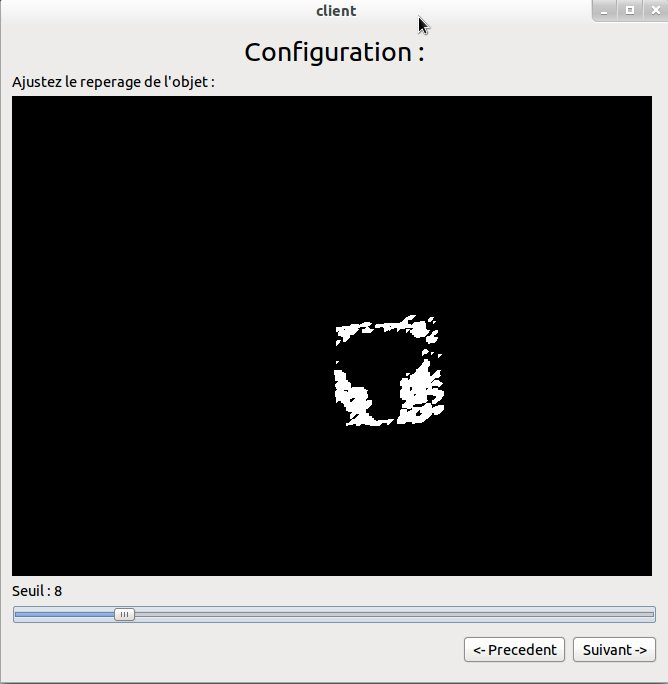
\includegraphics[scale=0.25]{capture1.jpg}
			\end{center}
		\end{frame}

		\begin{frame}{Suivi par couleur : Composantes connexes}
			\begin{itemize}
				\item{Calcul des différentes composantes connexes sur l'image binaire}
				\item{Sélection de la composante correspondant au curseur}
				\item{Récupération de son barycentre} 
			\end{itemize}
		\end{frame}

		\subsection{Suivi par Forme}
		\begin{frame}{Étalonnage par forme}
			\begin{itemize}
				\item{Sélection de la zone-objet}
				\item{Création d'une sous-image Template}
			\end{itemize}
		\end{frame}

		\begin{frame}{Suivi par forme}
			\begin{itemize}
				\item{Recherche du template dans l'image}
				\item{Sélection de la zone avec la meilleure correspondance}
			\end{itemize}
		\end{frame}
		\subsection{Comparatifs}
		\begin{frame}{Comparatif Couleur/Forme}
		\pause
			\begin{block}{Couleur}
				Avantages \\
				- Suivi rapide \\
				- Diversité possible de curseurs \\
				Faiblesses \\
				- Sensibilité à l'environnement\\
				- Dépendant de la qualité du dispositif d'acquisition\\
			\end{block}
			\pause
			\begin{block}{Forme}
				Avantages \\
				- Suivi moins dépendant de la qualité de l'environnement \\
				- Efficace sur des objets 'complexes'\\
				Faiblesses \\
				- Suivi  lent \\
				- Très sensible aux variations du curseur\\
			\end{block}
		\end{frame}
		\begin{frame}{Comparatif Simple/composante connexe}
		\pause
			\begin{block}{Barycentre simple}
				Avantages \\
				- Suivi rapide \\
				Faiblesses \\
				- Sensibilité aux parasites (fausses détections)\\
				- Précision fortement dépendante de l'environnement\\
			\end{block}
			\pause
			\begin{block}{Barycentre composante connexe}
				Avantages \\
				- Suivi plus précis \\
				- Résistance aux parasites \\
				Faiblesses \\
				- Suivi plus lent \\
				- Perte occasionnelle du curseur
			\end{block}
		\end{frame}

		\begin{frame}{Bilan}
			\begin{exampleblock}{Objectifs atteints}
				\begin{itemize}
				\item Bibliothèque utilisable et proposant plusieurs solutions de suivi
				\item Détection d'action implémentée dans deux des trois solutions
				\item Utilisation simple sans connaissances en traitement d'images
				\end{itemize}
			\end{exampleblock}
			\pause
			\begin{alertblock}{Difficultés et ouverture}
				\begin{itemize}
				\item Exploitation des bibliothèques OpenCv et CvBlob 
				\item Implémentation de la détection pour le suivi par forme
				\item Ajout à la bibliothèque de nouvelles fonctions de suivi
				\end{itemize}
			\end{alertblock}
		\end{frame}
	
	% Baptiste et Julien
	% Julien
	\section{Application}
		\begin{frame}{Architecture}
			\begin{block}{Objectifs de l'architecture conçue}
				\begin{itemize}
				\item{Avoir une application modulable et facilement extensible}
				\item{Fonctionnement identique pour les classes principales en réseau ou en local}
				\item{Pouvoir rajouter facilement des outils (pinceaux, gomme, etc.)}
				\item{Séparer le traitement du rendu}
				\end{itemize}
			\end{block}
		\end{frame}
		
		\begin{frame}{Diagramme de classes}
			\begin{center}		
			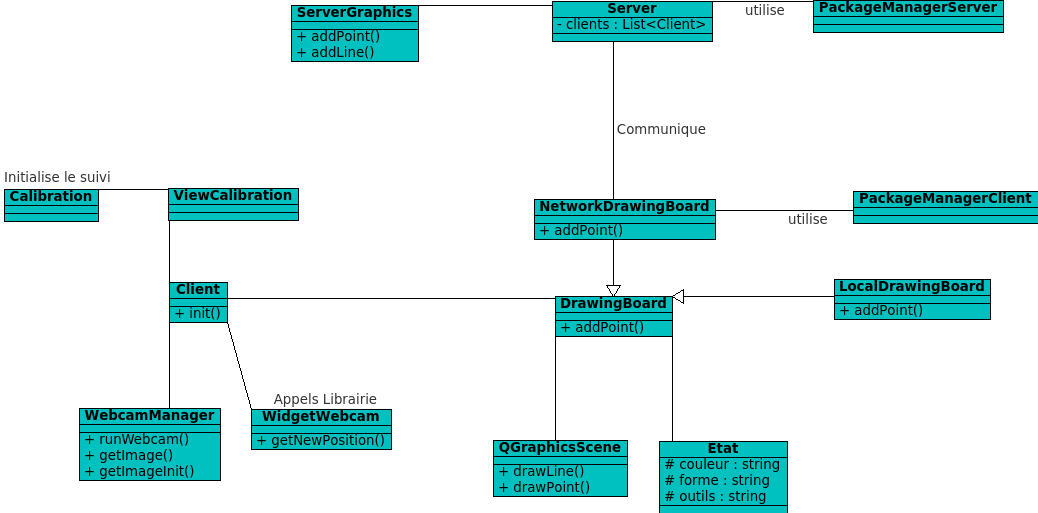
\includegraphics[scale=0.45]{../uml/classes.png}
			\end{center}
		\end{frame}
		
	% Baptiste
		\begin{frame}{Application}
			
			L'application est utilisable en local et en réseau, avec un fonctionnement identique.
			
			Le dessin virtuel interactif propose différents outils :
			\begin{itemize}
			\item La possibilité de changer la couleur du pinceau
      \item Celle d'ajuster la taille du pinceau
			\item Une gomme
			\item Fonctionnalité permettant d'exporter le dessin
			\item Possibilité de nettoyer complètement le tableau
			\item Mode plein-écran avec le dessin uniquement (vidéoprojecteur)
			\item Utilisation simultanée par plusieurs utilisateurs
			\item Application traduite et packagée (en .deb)
			\end{itemize}
		\end{frame}
		
	\subsection{Module Local}
		\begin{frame}{Fonctionnemment global}
			\begin{block}{Fonctionnement en local}
				\begin{itemize}
				\item Étalonnage selon la méthode voulue, choix du mode local
				\item Détection d'un mouvement, dessin directement sur le tableau en respectant les options
				\end{itemize}
			\end{block}
		\end{frame}
		
		\begin{frame}{Étalonnage}
			L'étalonnage se déroule en plusieurs phases.
			\begin{itemize}
			\item Choix de la webcam et de méthode de suivi
			\item Choix de l'objet à suivre à partir d'une photo, en l'entourant d'un rectangle
			\item Réglage du seuil de tolérance à partir du retour de l'étalonnage
			\item Choix du mode : réseau ou local
			\end{itemize}
		\end{frame}
		
		% TODO : compléter ou supprimer cette frame
		\begin{frame}{Utilisation de l'application}
		L'interface permets de visualiser le flux vidéo, et le dessin.
		
		Les mouvements sont détectés, et le dessin est effectué à partir de ces mouvements.
		\end{frame}
		
		% Bilan du projet côté interface
		\begin{frame}{Bilan}
			\begin{exampleblock}{Objectifs atteints}
				\begin{itemize}
				\item Application fonctionnelle et utilisable
				\item Beaucoup d'outils voulus implémentés
				\end{itemize}
			\end{exampleblock}
			\pause
			\begin{alertblock}{Difficultés et ouverture}
				\begin{itemize}
				\item Faire une interface gestuelle pour sélectionner gomme, couleur et forme
				\item Améliorer la gestion du dessin
				\item Relancer l'étalonnage sans relancer l'application
				\end{itemize}
			\end{alertblock}
		\end{frame}

	% Julien
	\subsection{Module Reseau}
		\begin{frame}{Fonctionnement global}
			\begin{block}{Fonctionnement en réseau}
				\begin{itemize}
				\item Étalonnage selon la méthode voulue, choix du mode réseau
				\item Récupération du dessin actuel par le client
				\item Détection d'un mouvement
				\item Envoi au serveur de ce mouvement (et des options) en respectant le protocole
				\item Réception du paquet côté serveur, dessin du serveur
				\item Envoi aux clients de ce point, avec les options (épaisseur, couleur)
				\item Réception côté client, et dessin en local
				\end{itemize}
			\end{block}
		\end{frame}
		
		\begin{frame}{Fonctionnemment global : schéma}
		
		Déroulement du fonctionnement en réseau de l'application :
			\begin{center}
			\scalebox{0.5}{% Graphic for TeX using PGF
% Title: /home/julien/master/projet/dessin-realite-augmentee/documents/uml/sequence_reseau.dia
% Creator: Dia v0.97.2
% CreationDate: Tue Apr 24 10:47:45 2012
% For: julien
% \usepackage{tikz}
% The following commands are not supported in PSTricks at present
% We define them conditionally, so when they are implemented,
% this pgf file will use them.
\ifx\du\undefined
  \newlength{\du}
\fi
\setlength{\du}{15\unitlength}
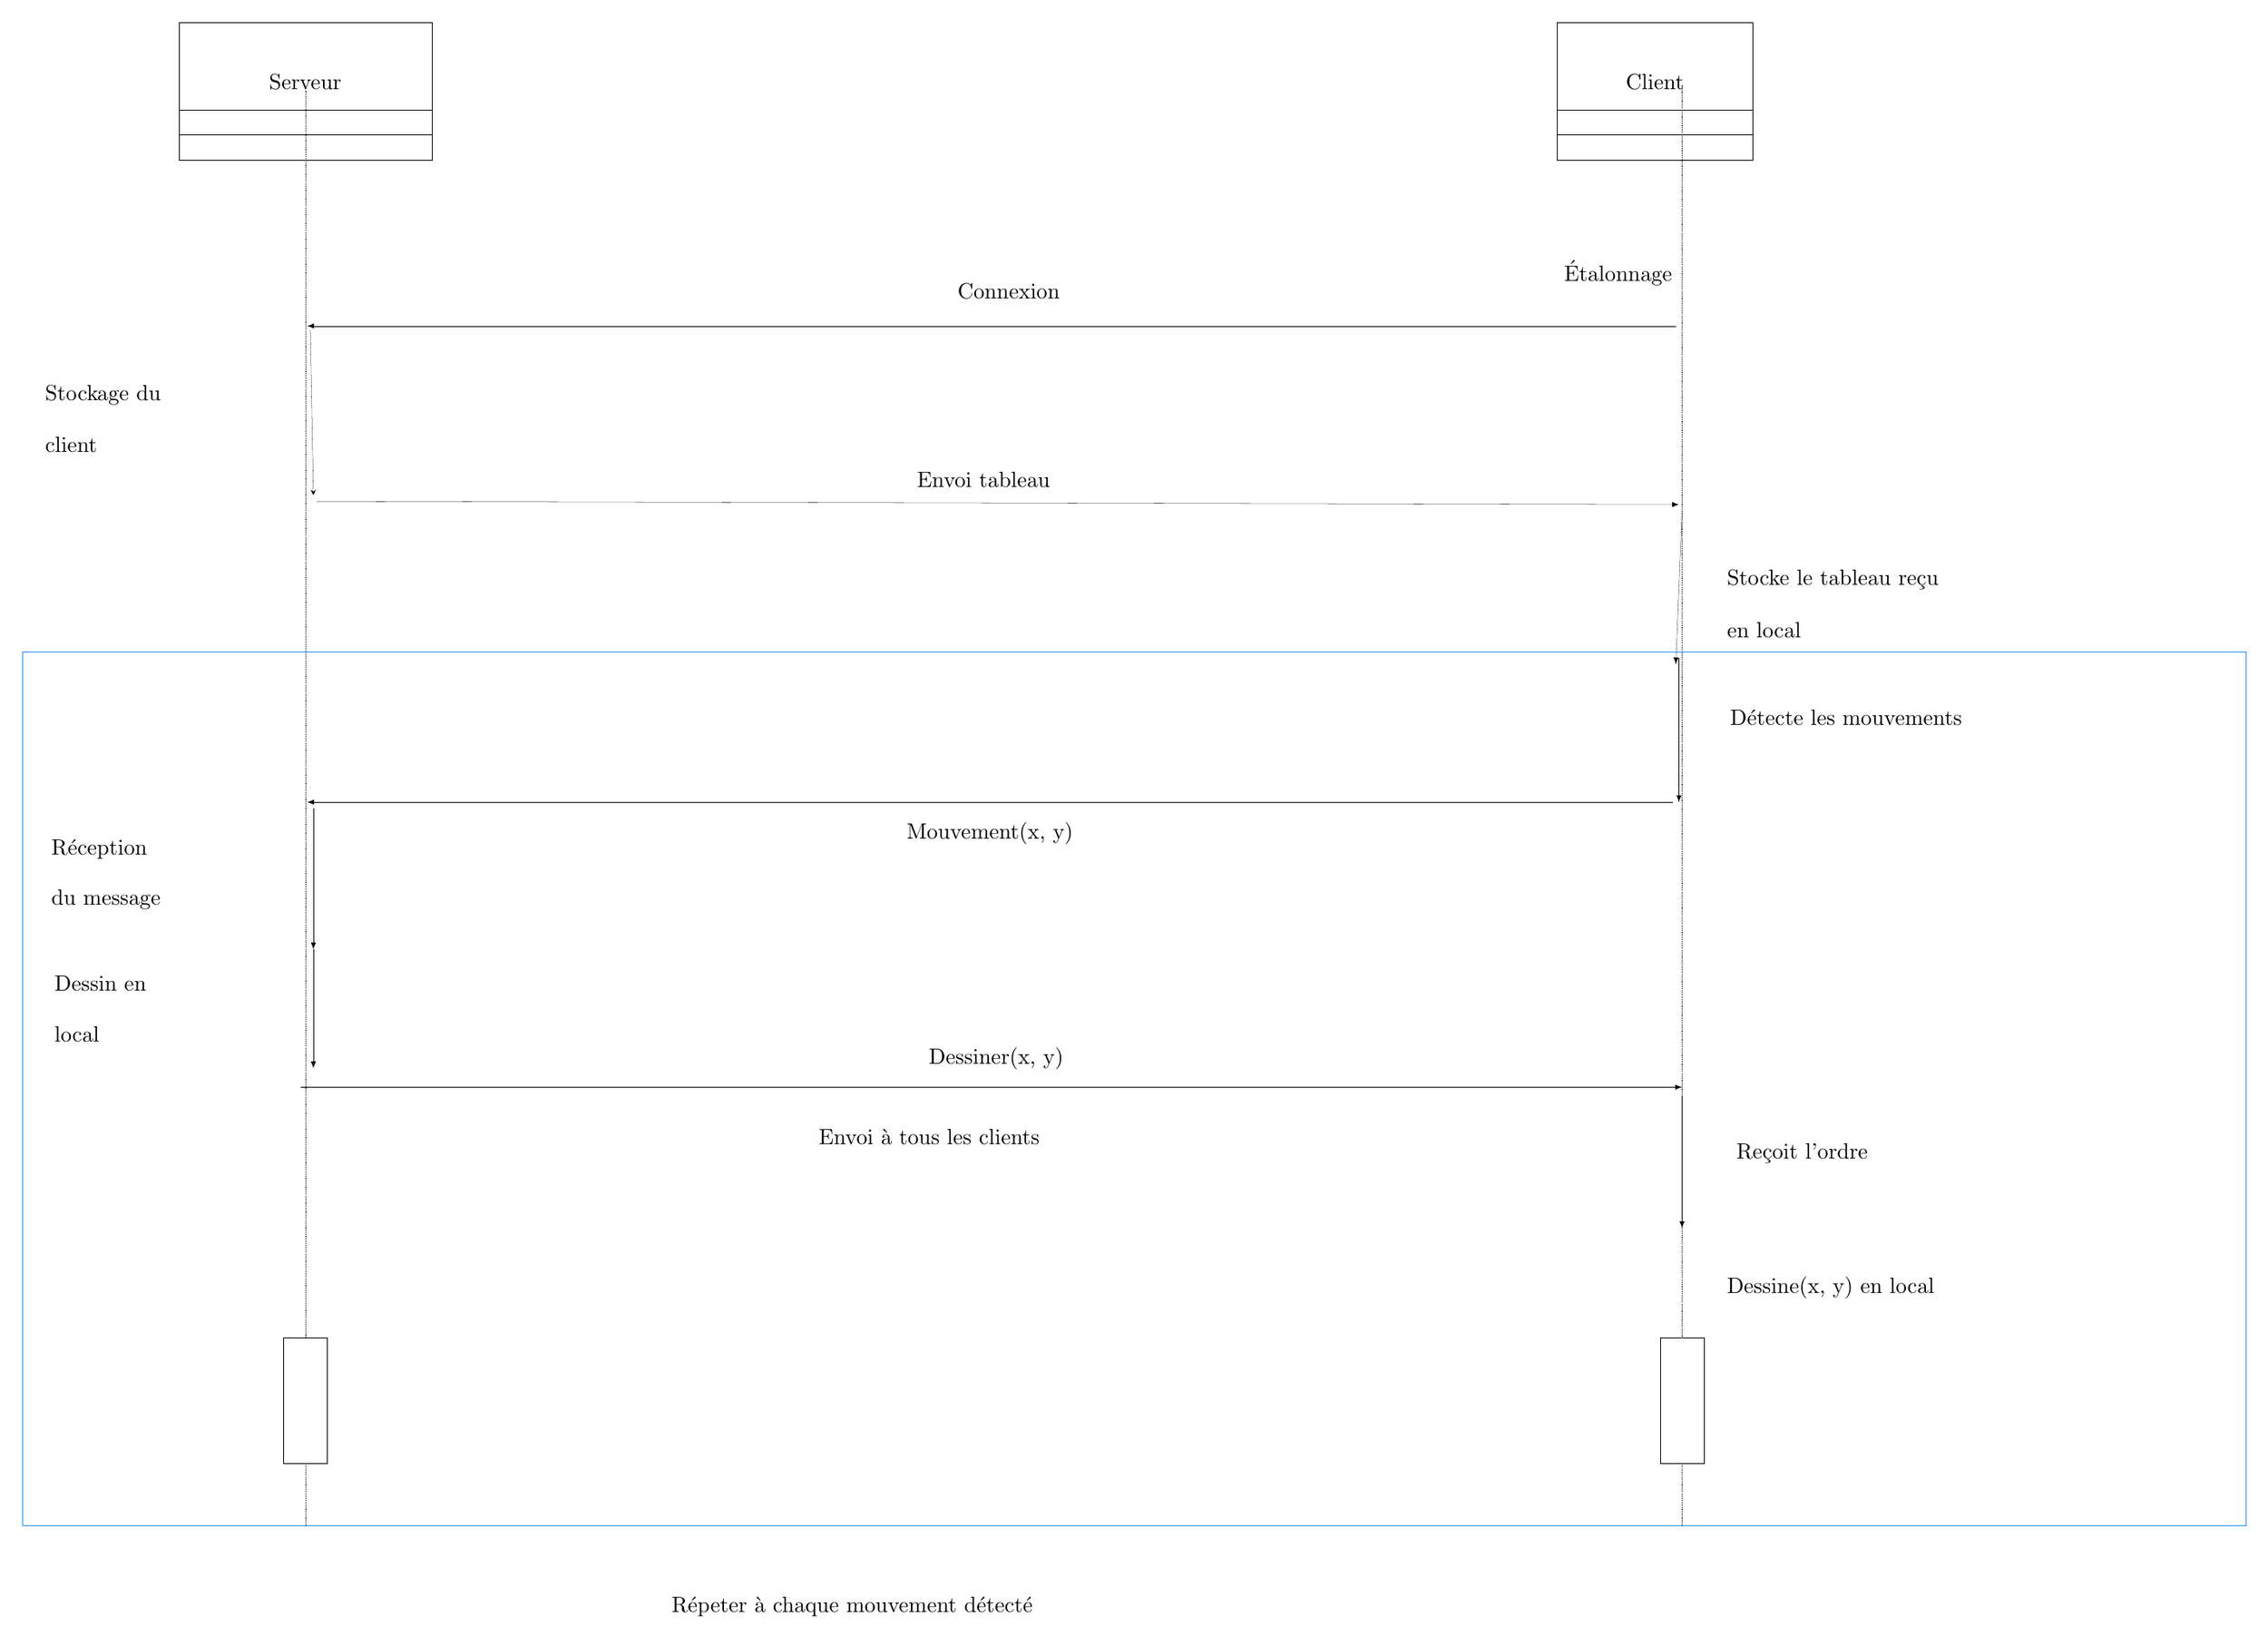
\begin{tikzpicture}
\pgftransformxscale{1.000000}
\pgftransformyscale{-1.000000}
\definecolor{dialinecolor}{rgb}{0.000000, 0.000000, 0.000000}
\pgfsetstrokecolor{dialinecolor}
\definecolor{dialinecolor}{rgb}{1.000000, 1.000000, 1.000000}
\pgfsetfillcolor{dialinecolor}
\pgfsetlinewidth{0.100000\du}
\pgfsetdash{}{0pt}
\definecolor{dialinecolor}{rgb}{1.000000, 1.000000, 1.000000}
\pgfsetfillcolor{dialinecolor}
\fill (5.000000\du,7.000000\du)--(5.000000\du,8.400000\du)--(9.042500\du,8.400000\du)--(9.042500\du,7.000000\du)--cycle;
\definecolor{dialinecolor}{rgb}{0.000000, 0.000000, 0.000000}
\pgfsetstrokecolor{dialinecolor}
\draw (5.000000\du,7.000000\du)--(5.000000\du,8.400000\du)--(9.042500\du,8.400000\du)--(9.042500\du,7.000000\du)--cycle;
% setfont left to latex
\definecolor{dialinecolor}{rgb}{0.000000, 0.000000, 0.000000}
\pgfsetstrokecolor{dialinecolor}
\node at (7.021250\du,7.950000\du){Serveur};
\definecolor{dialinecolor}{rgb}{1.000000, 1.000000, 1.000000}
\pgfsetfillcolor{dialinecolor}
\fill (5.000000\du,8.400000\du)--(5.000000\du,8.800000\du)--(9.042500\du,8.800000\du)--(9.042500\du,8.400000\du)--cycle;
\definecolor{dialinecolor}{rgb}{0.000000, 0.000000, 0.000000}
\pgfsetstrokecolor{dialinecolor}
\draw (5.000000\du,8.400000\du)--(5.000000\du,8.800000\du)--(9.042500\du,8.800000\du)--(9.042500\du,8.400000\du)--cycle;
\definecolor{dialinecolor}{rgb}{1.000000, 1.000000, 1.000000}
\pgfsetfillcolor{dialinecolor}
\fill (5.000000\du,8.800000\du)--(5.000000\du,9.200000\du)--(9.042500\du,9.200000\du)--(9.042500\du,8.800000\du)--cycle;
\definecolor{dialinecolor}{rgb}{0.000000, 0.000000, 0.000000}
\pgfsetstrokecolor{dialinecolor}
\draw (5.000000\du,8.800000\du)--(5.000000\du,9.200000\du)--(9.042500\du,9.200000\du)--(9.042500\du,8.800000\du)--cycle;
\pgfsetlinewidth{0.100000\du}
\pgfsetdash{}{0pt}
\definecolor{dialinecolor}{rgb}{1.000000, 1.000000, 1.000000}
\pgfsetfillcolor{dialinecolor}
\fill (27.000000\du,7.000000\du)--(27.000000\du,8.400000\du)--(30.132500\du,8.400000\du)--(30.132500\du,7.000000\du)--cycle;
\definecolor{dialinecolor}{rgb}{0.000000, 0.000000, 0.000000}
\pgfsetstrokecolor{dialinecolor}
\draw (27.000000\du,7.000000\du)--(27.000000\du,8.400000\du)--(30.132500\du,8.400000\du)--(30.132500\du,7.000000\du)--cycle;
% setfont left to latex
\definecolor{dialinecolor}{rgb}{0.000000, 0.000000, 0.000000}
\pgfsetstrokecolor{dialinecolor}
\node at (28.566250\du,7.950000\du){Client};
\definecolor{dialinecolor}{rgb}{1.000000, 1.000000, 1.000000}
\pgfsetfillcolor{dialinecolor}
\fill (27.000000\du,8.400000\du)--(27.000000\du,8.800000\du)--(30.132500\du,8.800000\du)--(30.132500\du,8.400000\du)--cycle;
\definecolor{dialinecolor}{rgb}{0.000000, 0.000000, 0.000000}
\pgfsetstrokecolor{dialinecolor}
\draw (27.000000\du,8.400000\du)--(27.000000\du,8.800000\du)--(30.132500\du,8.800000\du)--(30.132500\du,8.400000\du)--cycle;
\definecolor{dialinecolor}{rgb}{1.000000, 1.000000, 1.000000}
\pgfsetfillcolor{dialinecolor}
\fill (27.000000\du,8.800000\du)--(27.000000\du,9.200000\du)--(30.132500\du,9.200000\du)--(30.132500\du,8.800000\du)--cycle;
\definecolor{dialinecolor}{rgb}{0.000000, 0.000000, 0.000000}
\pgfsetstrokecolor{dialinecolor}
\draw (27.000000\du,8.800000\du)--(27.000000\du,9.200000\du)--(30.132500\du,9.200000\du)--(30.132500\du,8.800000\du)--cycle;
\pgfsetlinewidth{0.050000\du}
\pgfsetdash{}{0pt}
\pgfsetdash{{0.400000\du}{0.400000\du}}{0\du}
\definecolor{dialinecolor}{rgb}{0.000000, 0.000000, 0.000000}
\pgfsetstrokecolor{dialinecolor}
\draw (29.000000\du,8.000000\du)--(29.000000\du,28.000000\du);
\definecolor{dialinecolor}{rgb}{0.000000, 0.000000, 0.000000}
\pgfsetstrokecolor{dialinecolor}
\draw (29.000000\du,30.000000\du)--(29.000000\du,31.000000\du);
\pgfsetlinewidth{0.100000\du}
\pgfsetdash{}{0pt}
\definecolor{dialinecolor}{rgb}{1.000000, 1.000000, 1.000000}
\pgfsetfillcolor{dialinecolor}
\fill (28.650000\du,28.000000\du)--(28.650000\du,30.000000\du)--(29.350000\du,30.000000\du)--(29.350000\du,28.000000\du)--cycle;
\definecolor{dialinecolor}{rgb}{0.000000, 0.000000, 0.000000}
\pgfsetstrokecolor{dialinecolor}
\draw (28.650000\du,28.000000\du)--(28.650000\du,30.000000\du)--(29.350000\du,30.000000\du)--(29.350000\du,28.000000\du)--cycle;
\pgfsetlinewidth{0.050000\du}
\pgfsetdash{}{0pt}
\pgfsetdash{{0.400000\du}{0.400000\du}}{0\du}
\definecolor{dialinecolor}{rgb}{0.000000, 0.000000, 0.000000}
\pgfsetstrokecolor{dialinecolor}
\draw (7.021250\du,8.100000\du)--(7.021250\du,28.000000\du);
\definecolor{dialinecolor}{rgb}{0.000000, 0.000000, 0.000000}
\pgfsetstrokecolor{dialinecolor}
\draw (7.021250\du,30.000000\du)--(7.021250\du,31.000000\du);
\pgfsetlinewidth{0.100000\du}
\pgfsetdash{}{0pt}
\definecolor{dialinecolor}{rgb}{1.000000, 1.000000, 1.000000}
\pgfsetfillcolor{dialinecolor}
\fill (6.671250\du,28.000000\du)--(6.671250\du,30.000000\du)--(7.371250\du,30.000000\du)--(7.371250\du,28.000000\du)--cycle;
\definecolor{dialinecolor}{rgb}{0.000000, 0.000000, 0.000000}
\pgfsetstrokecolor{dialinecolor}
\draw (6.671250\du,28.000000\du)--(6.671250\du,30.000000\du)--(7.371250\du,30.000000\du)--(7.371250\du,28.000000\du)--cycle;
\pgfsetlinewidth{0.100000\du}
\pgfsetbuttcap
\pgfsetdash{}{0pt}
{
\definecolor{dialinecolor}{rgb}{0.000000, 0.000000, 0.000000}
\pgfsetfillcolor{dialinecolor}
% was here!!!
\pgfsetarrowsstart{latex}
\definecolor{dialinecolor}{rgb}{0.000000, 0.000000, 0.000000}
\pgfsetstrokecolor{dialinecolor}
\draw (7.050000\du,11.850000\du)--(28.900000\du,11.850000\du);
}
% setfont left to latex
\definecolor{dialinecolor}{rgb}{0.000000, 0.000000, 0.000000}
\pgfsetstrokecolor{dialinecolor}
\node at (18.250000\du,11.300000\du){Connexion};
\pgfsetlinewidth{0.100000\du}
\pgfsetdash{}{0pt}
\pgfsetdash{}{0pt}
\pgfsetbuttcap
{
\definecolor{dialinecolor}{rgb}{0.000000, 0.000000, 0.000000}
\pgfsetfillcolor{dialinecolor}
% was here!!!
\pgfsetarrowsend{stealth}
\definecolor{dialinecolor}{rgb}{0.000000, 0.000000, 0.000000}
\pgfsetstrokecolor{dialinecolor}
\draw (7.100000\du,11.900000\du)--(7.150000\du,14.550000\du);
}
\pgfsetlinewidth{0.100000\du}
\pgfsetbuttcap
\pgfsetdash{}{0pt}
{
\definecolor{dialinecolor}{rgb}{0.000000, 0.000000, 0.000000}
\pgfsetfillcolor{dialinecolor}
% was here!!!
\pgfsetarrowsstart{latex}
\definecolor{dialinecolor}{rgb}{0.000000, 0.000000, 0.000000}
\pgfsetstrokecolor{dialinecolor}
\draw (28.950000\du,14.700000\du)--(7.200000\du,14.650000\du);
}
% setfont left to latex
\definecolor{dialinecolor}{rgb}{0.000000, 0.000000, 0.000000}
\pgfsetstrokecolor{dialinecolor}
\node at (17.850000\du,14.300000\du){Envoi tableau};
% setfont left to latex
\definecolor{dialinecolor}{rgb}{0.000000, 0.000000, 0.000000}
\pgfsetstrokecolor{dialinecolor}
\node[anchor=west] at (27.000000\du,11.000000\du){Étalonnage};
% setfont left to latex
\definecolor{dialinecolor}{rgb}{0.000000, 0.000000, 0.000000}
\pgfsetstrokecolor{dialinecolor}
\node[anchor=west] at (2.750000\du,12.950000\du){Stockage du };
% setfont left to latex
\definecolor{dialinecolor}{rgb}{0.000000, 0.000000, 0.000000}
\pgfsetstrokecolor{dialinecolor}
\node[anchor=west] at (2.750000\du,13.750000\du){client};
\pgfsetlinewidth{0.100000\du}
\pgfsetbuttcap
\pgfsetdash{}{0pt}
{
\definecolor{dialinecolor}{rgb}{0.000000, 0.000000, 0.000000}
\pgfsetfillcolor{dialinecolor}
% was here!!!
\pgfsetarrowsstart{latex}
\definecolor{dialinecolor}{rgb}{0.000000, 0.000000, 0.000000}
\pgfsetstrokecolor{dialinecolor}
\draw (28.900000\du,17.250000\du)--(29.000000\du,14.800000\du);
}
% setfont left to latex
% setfont left to latex
\definecolor{dialinecolor}{rgb}{0.000000, 0.000000, 0.000000}
\pgfsetstrokecolor{dialinecolor}
\node[anchor=west] at (29.600000\du,15.900000\du){Stocke le tableau reçu};
% setfont left to latex
\definecolor{dialinecolor}{rgb}{0.000000, 0.000000, 0.000000}
\pgfsetstrokecolor{dialinecolor}
\node[anchor=west] at (29.600000\du,16.700000\du){en local};
\pgfsetlinewidth{0.100000\du}
\pgfsetbuttcap
\pgfsetdash{}{0pt}
{
\definecolor{dialinecolor}{rgb}{0.000000, 0.000000, 0.000000}
\pgfsetfillcolor{dialinecolor}
% was here!!!
\pgfsetarrowsstart{latex}
\definecolor{dialinecolor}{rgb}{0.000000, 0.000000, 0.000000}
\pgfsetstrokecolor{dialinecolor}
\draw (7.050000\du,19.450000\du)--(28.850000\du,19.450000\du);
}
% setfont left to latex
\definecolor{dialinecolor}{rgb}{0.000000, 0.000000, 0.000000}
\pgfsetstrokecolor{dialinecolor}
\node at (17.950000\du,19.950000\du){Mouvement(x, y)};
% setfont left to latex
\definecolor{dialinecolor}{rgb}{0.000000, 0.000000, 0.000000}
\pgfsetstrokecolor{dialinecolor}
\node[anchor=west] at (2.850000\du,20.200000\du){Réception };
% setfont left to latex
\definecolor{dialinecolor}{rgb}{0.000000, 0.000000, 0.000000}
\pgfsetstrokecolor{dialinecolor}
\node[anchor=west] at (2.850000\du,21.000000\du){du message};
% setfont left to latex
\definecolor{dialinecolor}{rgb}{0.000000, 0.000000, 0.000000}
\pgfsetstrokecolor{dialinecolor}
\node[anchor=west] at (2.900000\du,22.350000\du){Dessin en};
% setfont left to latex
\definecolor{dialinecolor}{rgb}{0.000000, 0.000000, 0.000000}
\pgfsetstrokecolor{dialinecolor}
\node[anchor=west] at (2.900000\du,23.150000\du){local};
\pgfsetlinewidth{0.100000\du}
\pgfsetbuttcap
\pgfsetdash{}{0pt}
{
\definecolor{dialinecolor}{rgb}{0.000000, 0.000000, 0.000000}
\pgfsetfillcolor{dialinecolor}
% was here!!!
\pgfsetarrowsstart{latex}
\definecolor{dialinecolor}{rgb}{0.000000, 0.000000, 0.000000}
\pgfsetstrokecolor{dialinecolor}
\draw (7.150000\du,21.800000\du)--(7.150000\du,19.550000\du);
}
% setfont left to latex
\pgfsetlinewidth{0.100000\du}
\pgfsetbuttcap
\pgfsetdash{}{0pt}
{
\definecolor{dialinecolor}{rgb}{0.000000, 0.000000, 0.000000}
\pgfsetfillcolor{dialinecolor}
% was here!!!
\pgfsetarrowsstart{latex}
\definecolor{dialinecolor}{rgb}{0.000000, 0.000000, 0.000000}
\pgfsetstrokecolor{dialinecolor}
\draw (7.150000\du,23.700000\du)--(7.150000\du,21.800000\du);
}
% setfont left to latex
\pgfsetlinewidth{0.100000\du}
\pgfsetbuttcap
\pgfsetdash{}{0pt}
{
\definecolor{dialinecolor}{rgb}{0.000000, 0.000000, 0.000000}
\pgfsetfillcolor{dialinecolor}
% was here!!!
\pgfsetarrowsstart{latex}
\definecolor{dialinecolor}{rgb}{0.000000, 0.000000, 0.000000}
\pgfsetstrokecolor{dialinecolor}
\draw (28.950000\du,19.450000\du)--(28.950000\du,17.150000\du);
}
% setfont left to latex
% setfont left to latex
\definecolor{dialinecolor}{rgb}{0.000000, 0.000000, 0.000000}
\pgfsetstrokecolor{dialinecolor}
\node[anchor=west] at (29.650000\du,18.100000\du){Détecte les mouvements};
\pgfsetlinewidth{0.100000\du}
\pgfsetbuttcap
\pgfsetdash{}{0pt}
{
\definecolor{dialinecolor}{rgb}{0.000000, 0.000000, 0.000000}
\pgfsetfillcolor{dialinecolor}
% was here!!!
\pgfsetarrowsstart{latex}
\definecolor{dialinecolor}{rgb}{0.000000, 0.000000, 0.000000}
\pgfsetstrokecolor{dialinecolor}
\draw (29.000000\du,24.000000\du)--(6.950000\du,24.000000\du);
}
% setfont left to latex
\definecolor{dialinecolor}{rgb}{0.000000, 0.000000, 0.000000}
\pgfsetstrokecolor{dialinecolor}
\node at (18.050000\du,23.550000\du){Dessiner(x, y)};
% setfont left to latex
\definecolor{dialinecolor}{rgb}{0.000000, 0.000000, 0.000000}
\pgfsetstrokecolor{dialinecolor}
\node[anchor=west] at (15.100000\du,24.800000\du){Envoi à tous les clients};
\pgfsetlinewidth{0.100000\du}
\pgfsetbuttcap
\pgfsetdash{}{0pt}
{
\definecolor{dialinecolor}{rgb}{0.000000, 0.000000, 0.000000}
\pgfsetfillcolor{dialinecolor}
% was here!!!
\pgfsetarrowsstart{latex}
\definecolor{dialinecolor}{rgb}{0.000000, 0.000000, 0.000000}
\pgfsetstrokecolor{dialinecolor}
\draw (29.000000\du,26.250000\du)--(29.000000\du,24.150000\du);
}
% setfont left to latex
% setfont left to latex
\definecolor{dialinecolor}{rgb}{0.000000, 0.000000, 0.000000}
\pgfsetstrokecolor{dialinecolor}
\node[anchor=west] at (29.750000\du,25.050000\du){Reçoit l'ordre};
% setfont left to latex
\definecolor{dialinecolor}{rgb}{0.000000, 0.000000, 0.000000}
\pgfsetstrokecolor{dialinecolor}
\node[anchor=west] at (29.600000\du,27.200000\du){Dessine(x, y) en local};
\pgfsetlinewidth{0.100000\du}
\pgfsetdash{}{0pt}
\pgfsetdash{}{0pt}
\pgfsetmiterjoin
\definecolor{dialinecolor}{rgb}{0.117647, 0.564706, 1.000000}
\pgfsetstrokecolor{dialinecolor}
\draw (2.500000\du,17.050000\du)--(2.500000\du,31.000000\du)--(38.000000\du,31.000000\du)--(38.000000\du,17.050000\du)--cycle;
% setfont left to latex
\definecolor{dialinecolor}{rgb}{0.117647, 0.564706, 1.000000}
\pgfsetstrokecolor{dialinecolor}
\node[anchor=west] at (12.750000\du,32.300000\du){Répeter à chaque mouvement détecté};
\end{tikzpicture}
} 
			\end{center}
		\end{frame}
		
		% Bilan de l'application côté réseau
		\begin{frame}{Bilan}
			\begin{exampleblock}{Objectifs atteints}
				\begin{itemize}
				\item Architecture identique au fonctionnement en local
				\item Application fonctionnelle en mode réseau malgré la difficulté
				\item Tous les outils fonctionnent
				\end{itemize}
			\end{exampleblock}
			\pause
			\begin{alertblock}{Difficultés et ouverture}
				\begin{itemize}
				\item Optimiser fortement le mode réseau pour réduire les problèmes de lenteur
				\item Mettre par défaut une couleur à chaque utilisateur
				\end{itemize}
			\end{alertblock}
		\end{frame}

	\section{Conclusion}
		\begin{frame}{Conclusion}
			\begin{exampleblock}{Objectifs atteints}
				- Solution fonctionnelle \\
				- Respect du cahier des charges \\
				- Découverte (Technologies, gestion de projet...) \\ 
			\end{exampleblock}
			\pause
			\begin{alertblock}{Difficultés}
				- Collaboration : Développement incrémental qui oblige à beaucoup communiquer \\
				- Formation : Traitement de l'image, Conception d'architectures \\
				- Techniques : Architecture, Fuites de mémoire...\\
			\end{alertblock}
			\pause
			\begin{block}{Ouverture}
				- Diversifier et optimiser les méthodes de suivi \\
				- Rajouter des fonctionnalités côté application \\
			\end{block}
		\end{frame}
	
	\begin{frame}{Sources et bibliographie}
  http://www.sciencedirect.com.www.ezp.biu-montpellier.fr/science/article/pii/S026288561100120X \\
  http://www.irit.fr/recherches/SAMOVA/pageAnalysis.html\\
  http://www.irit.fr/~Philippe.Joly/Teaching/L3SI/ti.html\\
  http://opencv.willowgarage.com/wiki/\\
  code.google.com/p/cvblob/ 
	\end{frame}

\end{document}
